\documentclass[border=10pt]{standalone}
\usepackage{tikz}
\usetikzlibrary{shapes, arrows.meta, positioning, calc, fit, backgrounds, shadows}

\begin{document}
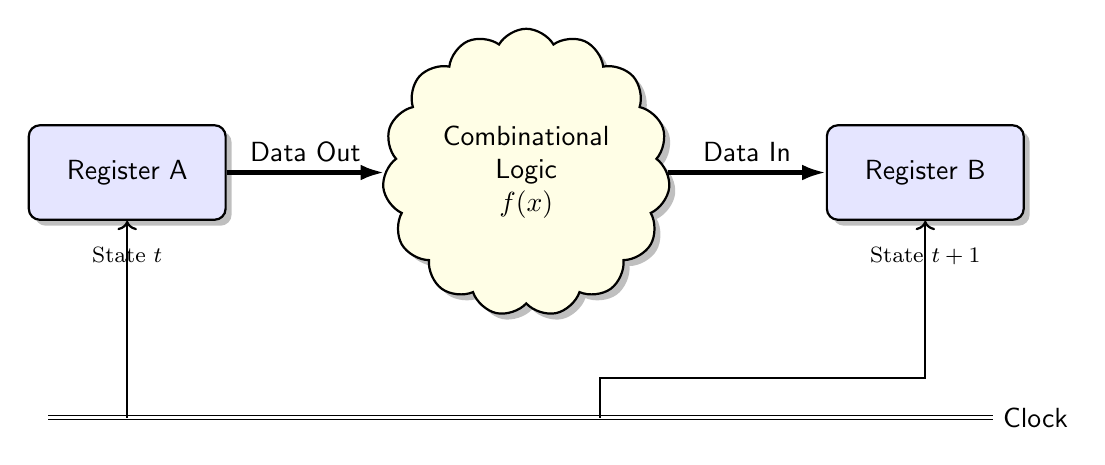
\begin{tikzpicture}[
    font=\sffamily,
    thick,
    reg/.style={draw, rounded corners, minimum width=2.5cm, minimum height=1.2cm, align=center, fill=blue!10, drop shadow},
    logic/.style={draw, cloud, cloud puffs=15, cloud puff arc=120, minimum width=3.5cm, minimum height=2cm, align=center, fill=yellow!10, drop shadow},
    arrow/.style={-{Latex[length=3mm, width=2mm]}, line width=1.5pt},
    clock_line/.style={thin, double, double distance=1pt},
    label_text/.style={font=\small, align=center}
]

    % Components
    \node[reg] (reg_a) {Register A};
    \node[logic, right=2cm of reg_a] (comb_logic) {Combinational\\Logic\\$f(x)$};
    \node[reg, right=2cm of comb_logic] (reg_b) {Register B};

    % Connections
    \draw[arrow] (reg_a) -- node[above] {Data Out} (comb_logic);
    \draw[arrow] (comb_logic) -- node[above] {Data In} (reg_b);

    % Clock signal
    \coordinate (clk_start) at ($(reg_a.south) + (-1, -2.5)$);
    \draw[clock_line] (clk_start) -- ++(12,0) node[right] {Clock};
    
    \draw[->] ($(clk_start) + (1,0)$) -- ++(0, 0.5) -| (reg_a.south);
    \draw[->] ($(clk_start) + (7,0)$) -- ++(0, 0.5) -| (reg_b.south);

    % Feedback Loop description (optional dashed line to imply sequence)
    %\draw[dashed, ->, gray] (reg_b.north) to[bend right=30] (reg_a.north);

    % Annotations
    \node[below=0.2cm of reg_a, font=\footnotesize] {State $t$};
    \node[below=0.2cm of reg_b, font=\footnotesize] {State $t+1$};

\end{tikzpicture}
\end{document}
